\documentclass[11pt,letterpaper]{article}
\usepackage{fullpage}
\usepackage[top=1.75cm, bottom=4cm, left=1.25cm, right=1.25cm]{geometry}
\usepackage{amsmath,amsthm,amsfonts,amssymb,amscd}
\usepackage{lastpage}
\usepackage{enumerate}
\usepackage{fancyhdr}
\usepackage{mathrsfs}
\usepackage{xcolor}
\usepackage{graphicx}
\usepackage{listings}
\usepackage{hyperref}
\usepackage{tcolorbox}
\usepackage{bbm}
\usepackage{cite}
\usepackage[numbers]{natbib}

\usepackage[utf8]{inputenc}
\usepackage{amsmath, amsfonts, mathrsfs}
\usepackage{enumitem}
\usepackage{wrapfig}
\usepackage{graphicx}
\usepackage{hyperref}
\usepackage{indentfirst}
\usepackage{placeins}
\usepackage{xcolor}
\usepackage{comment}
\usepackage{float}

\hypersetup{%
colorlinks=true,
urlcolor=blue,
citecolor=blue
}

\renewcommand\lstlistingname{Algorithm}
\renewcommand\lstlistlistingname{Algorithms}
\def\lstlistingautorefname{Alg.}

\lstdefinestyle{Python}{
  language        = Python,
  frame           = lines,
  basicstyle      = \footnotesize,
  keywordstyle    = \color{blue},
  stringstyle     = \color{green},
  commentstyle    = \color{red}\ttfamily
}

\setlength{\parindent}{0.0in}
\setlength{\parskip}{0.05in}

\newtcolorbox{cbox}[3][]
{
  colframe = #2!25,
  colback  = #2!10,
  coltitle = #2!20!black,
  title    = {#3},
  #1,
}

\newcommand\course{CS 674}
\newcommand\instructor{Dr. Wingate}
\newcommand\name{Jake Callahan, Taylor Paskett}

\pagestyle{fancyplain}
\headheight 32pt
\lhead{\name \\ \today}
\chead{\textbf{}}
\rhead{\course \\ \instructor}
\lfoot{}
\cfoot{}
\rfoot{\small\thepage}
\headsep 1.5em

\title{Gaussian Process Guided Neural Networks: An Exploration}
\author{\name}

\begin{document}

\maketitle
Things to talk about:
\begin{itemize}
  \item What does Gaussian process bring to the table that regular NN's lack?
  \item Why is using a GPGNN a good idea? What does it do to the model? i.e. a PGNN helps ensure results stay phsyically consistent
  \item data
  \item Model architecture: based off Whenet, etc
  \item novel loss function
  \item how we trained
  \item results
\section{Introduction}
  A major problem facing neural networks today is the size of their required training set. Neural networks need a large amount of data to train an accurate model. Further, neural networks can only learn relationships that exist in these data, and aren't well-suited to ingesting and learning from prior knowledge about the data.

  Conversely, many Bayesian inference- based statistical methods are well-suited for training with smaller amounts of data and rely on imposed prior knowledge. However, they suffer from infeasibility at large scales and lack versatility across problem types.

  We propose a network architecture that combines the strengths of these models and mitigates their weaknesses.
  Inspired by physics-guided neural networks (PGNN), which rely on physical models to guide the training of the neural network \cite{PGNN}, we create a similar that uses a Gaussian process to guide the training of a conventional neural network. {\color{red} CONFIRM: In this paper, we show that on a face-pose detection problem, the Gaussian Process Guided Neural Network (GPNN) achieves similar results to the current  state-of-the-art \cite{whenet} while using less data.}

\section{Regular model vs. GPGNN}

\section{Data}
  We apply our GPGNN model to a common problem: facial pose detection. Specifically, we use the 300W-LP dataset \cite{300wlp}. This dataset is composed of one input variable, a close-up facial image, and three outcome variables which define the facial pose: pitch, yaw, and roll. These pose parameters are given in degrees, and range from $-90^{\circ}$ to $90^{\circ}$. This dataset is widely used in face-pose estimation problems and as such is a natural choice for training the GPGNN.

\section{Architecture}
  \subsection{WHENet}
    We base our model architecture on Zhou and Gregson's WHENet model \cite{whenet}. This model is the current state-of-the art, and will be used as a baseline comparison for the success of our GPGNN. WHENet is an extension of the successful EfficientNet model developed by Tan and Le \cite{efn}. WHENet uses EfficientNet as its first layer. It then takes the EfficientNet outputs and applies two separate loss functions to each of the yaw, pitch, and roll.

    One loss function is a mean-squared error loss that measures the model's regression performance, and the other is a cross-entropy loss that measures how well the model would do if it were a classification problem. This cross-entropy loss is applied by first binning each of the yaw, pitch and roll into $60$ bins of $3$ degrees each, and then feeding these bins to the cross-entropy loss function. The total loss of the model is the sum across all loss terms. See Figure~\ref{fig:whenet_architecture} (courtesy of \cite{whenet}) for a visualization of this architecture.
  \subsection{GPGNN}
    Our GPGNN architecture is highly similar. We


    \begin{figure}[!htb]
    \centering
       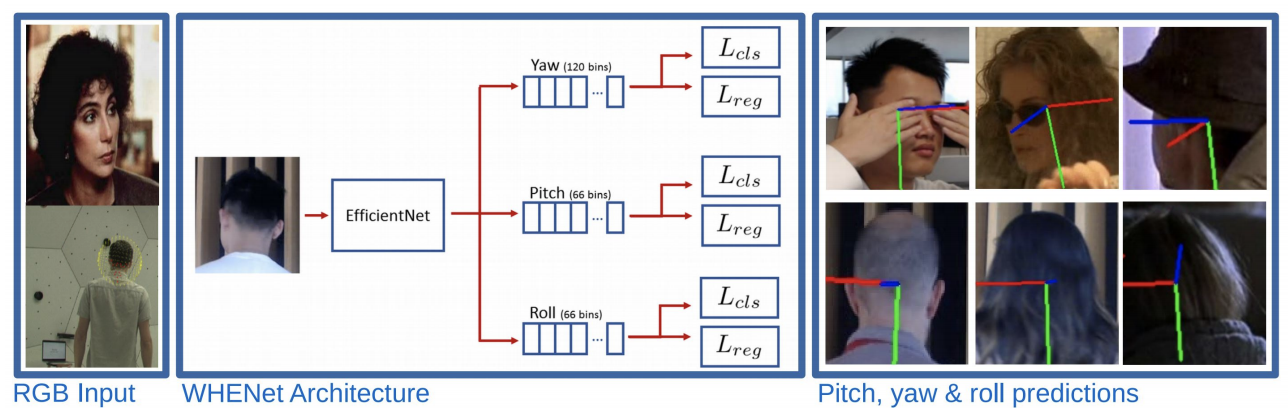
\includegraphics[width=0.65\linewidth]{./pics/whenet.png}
       \caption{Illustration of WHENet architecture}
       \label{fig:whenet_architecture}
    \end{figure}

\bibliography{references.bib}{}
\bibliographystyle{plainnat}

\end{document}
